% Options for packages loaded elsewhere
% Options for packages loaded elsewhere
\PassOptionsToPackage{unicode}{hyperref}
\PassOptionsToPackage{hyphens}{url}
\PassOptionsToPackage{dvipsnames,svgnames,x11names}{xcolor}
%
\documentclass[
  12pt,
  letterpaper,
  DIV=11,
  numbers=noendperiod]{scrartcl}
\usepackage{xcolor}
\usepackage{amsmath,amssymb}
\setcounter{secnumdepth}{-\maxdimen} % remove section numbering
\usepackage{iftex}
\ifPDFTeX
  \usepackage[T1]{fontenc}
  \usepackage[utf8]{inputenc}
  \usepackage{textcomp} % provide euro and other symbols
\else % if luatex or xetex
  \usepackage{unicode-math} % this also loads fontspec
  \defaultfontfeatures{Scale=MatchLowercase}
  \defaultfontfeatures[\rmfamily]{Ligatures=TeX,Scale=1}
\fi
\usepackage{lmodern}
\ifPDFTeX\else
  % xetex/luatex font selection
  \setmainfont[]{Times New Roman}
  \setmonofont[]{Courier New}
\fi
% Use upquote if available, for straight quotes in verbatim environments
\IfFileExists{upquote.sty}{\usepackage{upquote}}{}
\IfFileExists{microtype.sty}{% use microtype if available
  \usepackage[]{microtype}
  \UseMicrotypeSet[protrusion]{basicmath} % disable protrusion for tt fonts
}{}
\usepackage{setspace}
\makeatletter
\@ifundefined{KOMAClassName}{% if non-KOMA class
  \IfFileExists{parskip.sty}{%
    \usepackage{parskip}
  }{% else
    \setlength{\parindent}{0pt}
    \setlength{\parskip}{6pt plus 2pt minus 1pt}}
}{% if KOMA class
  \KOMAoptions{parskip=half}}
\makeatother
% Make \paragraph and \subparagraph free-standing
\makeatletter
\ifx\paragraph\undefined\else
  \let\oldparagraph\paragraph
  \renewcommand{\paragraph}{
    \@ifstar
      \xxxParagraphStar
      \xxxParagraphNoStar
  }
  \newcommand{\xxxParagraphStar}[1]{\oldparagraph*{#1}\mbox{}}
  \newcommand{\xxxParagraphNoStar}[1]{\oldparagraph{#1}\mbox{}}
\fi
\ifx\subparagraph\undefined\else
  \let\oldsubparagraph\subparagraph
  \renewcommand{\subparagraph}{
    \@ifstar
      \xxxSubParagraphStar
      \xxxSubParagraphNoStar
  }
  \newcommand{\xxxSubParagraphStar}[1]{\oldsubparagraph*{#1}\mbox{}}
  \newcommand{\xxxSubParagraphNoStar}[1]{\oldsubparagraph{#1}\mbox{}}
\fi
\makeatother


\usepackage{longtable,booktabs,array}
\usepackage{calc} % for calculating minipage widths
% Correct order of tables after \paragraph or \subparagraph
\usepackage{etoolbox}
\makeatletter
\patchcmd\longtable{\par}{\if@noskipsec\mbox{}\fi\par}{}{}
\makeatother
% Allow footnotes in longtable head/foot
\IfFileExists{footnotehyper.sty}{\usepackage{footnotehyper}}{\usepackage{footnote}}
\makesavenoteenv{longtable}
\usepackage{graphicx}
\makeatletter
\newsavebox\pandoc@box
\newcommand*\pandocbounded[1]{% scales image to fit in text height/width
  \sbox\pandoc@box{#1}%
  \Gscale@div\@tempa{\textheight}{\dimexpr\ht\pandoc@box+\dp\pandoc@box\relax}%
  \Gscale@div\@tempb{\linewidth}{\wd\pandoc@box}%
  \ifdim\@tempb\p@<\@tempa\p@\let\@tempa\@tempb\fi% select the smaller of both
  \ifdim\@tempa\p@<\p@\scalebox{\@tempa}{\usebox\pandoc@box}%
  \else\usebox{\pandoc@box}%
  \fi%
}
% Set default figure placement to htbp
\def\fps@figure{htbp}
\makeatother


% definitions for citeproc citations
\NewDocumentCommand\citeproctext{}{}
\NewDocumentCommand\citeproc{mm}{%
  \begingroup\def\citeproctext{#2}\cite{#1}\endgroup}
\makeatletter
 % allow citations to break across lines
 \let\@cite@ofmt\@firstofone
 % avoid brackets around text for \cite:
 \def\@biblabel#1{}
 \def\@cite#1#2{{#1\if@tempswa , #2\fi}}
\makeatother
\newlength{\cslhangindent}
\setlength{\cslhangindent}{1.5em}
\newlength{\csllabelwidth}
\setlength{\csllabelwidth}{3em}
\newenvironment{CSLReferences}[2] % #1 hanging-indent, #2 entry-spacing
 {\begin{list}{}{%
  \setlength{\itemindent}{0pt}
  \setlength{\leftmargin}{0pt}
  \setlength{\parsep}{0pt}
  % turn on hanging indent if param 1 is 1
  \ifodd #1
   \setlength{\leftmargin}{\cslhangindent}
   \setlength{\itemindent}{-1\cslhangindent}
  \fi
  % set entry spacing
  \setlength{\itemsep}{#2\baselineskip}}}
 {\end{list}}
\usepackage{calc}
\newcommand{\CSLBlock}[1]{\hfill\break\parbox[t]{\linewidth}{\strut\ignorespaces#1\strut}}
\newcommand{\CSLLeftMargin}[1]{\parbox[t]{\csllabelwidth}{\strut#1\strut}}
\newcommand{\CSLRightInline}[1]{\parbox[t]{\linewidth - \csllabelwidth}{\strut#1\strut}}
\newcommand{\CSLIndent}[1]{\hspace{\cslhangindent}#1}



\setlength{\emergencystretch}{3em} % prevent overfull lines

\providecommand{\tightlist}{%
  \setlength{\itemsep}{0pt}\setlength{\parskip}{0pt}}



 


\KOMAoption{captions}{tableheading}
\makeatletter
\@ifpackageloaded{caption}{}{\usepackage{caption}}
\AtBeginDocument{%
\ifdefined\contentsname
  \renewcommand*\contentsname{Table of contents}
\else
  \newcommand\contentsname{Table of contents}
\fi
\ifdefined\listfigurename
  \renewcommand*\listfigurename{List of Figures}
\else
  \newcommand\listfigurename{List of Figures}
\fi
\ifdefined\listtablename
  \renewcommand*\listtablename{List of Tables}
\else
  \newcommand\listtablename{List of Tables}
\fi
\ifdefined\figurename
  \renewcommand*\figurename{Figure}
\else
  \newcommand\figurename{Figure}
\fi
\ifdefined\tablename
  \renewcommand*\tablename{Table}
\else
  \newcommand\tablename{Table}
\fi
}
\@ifpackageloaded{float}{}{\usepackage{float}}
\floatstyle{ruled}
\@ifundefined{c@chapter}{\newfloat{codelisting}{h}{lop}}{\newfloat{codelisting}{h}{lop}[chapter]}
\floatname{codelisting}{Listing}
\newcommand*\listoflistings{\listof{codelisting}{List of Listings}}
\makeatother
\makeatletter
\makeatother
\makeatletter
\@ifpackageloaded{caption}{}{\usepackage{caption}}
\@ifpackageloaded{subcaption}{}{\usepackage{subcaption}}
\makeatother
\usepackage{bookmark}
\IfFileExists{xurl.sty}{\usepackage{xurl}}{} % add URL line breaks if available
\urlstyle{same}
\hypersetup{
  pdftitle={Final Project: Deep Learning for Breast Cancer Detection},
  pdfauthor={Takeshi Fujii, MD},
  colorlinks=true,
  linkcolor={blue},
  filecolor={Maroon},
  citecolor={Blue},
  urlcolor={Blue},
  pdfcreator={LaTeX via pandoc}}


\title{Final Project: Deep Learning for Breast Cancer Detection}
\author{Takeshi Fujii, MD \and }
\date{20 April 2025}
\begin{document}
\maketitle

\renewcommand*\contentsname{Table of contents}
{
\hypersetup{linkcolor=}
\setcounter{tocdepth}{3}
\tableofcontents
}

\setstretch{1.5}
\subsection{Abstract}\label{abstract}

\begin{itemize}
\tightlist
\item
  One-paragraph summary of the problem, dataset, methodology, and main
  findings.
\item
  One-paragraph summary of the problem, dataset, approach, and key
  results.
\end{itemize}

\subsection{1. Introduction}\label{introduction}

\subsubsection{1.1 Background \&
Motivation}\label{background-motivation}

\begin{itemize}
\tightlist
\item
  Describe the clinical and societal significance of early breast cancer
  detection.
\item
  Mention the NHS 2025 initiative and how AI fits into screening.
\end{itemize}

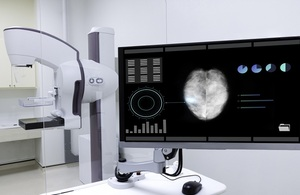
\includegraphics[width=0.5\linewidth,height=\textheight,keepaspectratio]{figures/mammogram.jpg}

According to recent research\textsuperscript{1}, neural networks
outperform \ldots{}

\subsubsection{1.2 Objectives}\label{objectives}

\begin{itemize}
\tightlist
\item
  Apply deep learning (CNNs) to mammography image classification.
\item
  Evaluate performance vs.~traditional methods/radiologists.
\end{itemize}

\subsubsection{1.3 Scope}\label{scope}

Briefly note focus on classification (benign vs malignant), dataset
used, and evaluation metrics.

Background \& Motivation

\begin{itemize}
\tightlist
\item
  Significance of early breast cancer detection.
\item
  NHS 2025 initiative on DL for screening.
\end{itemize}

Project Objectives

\begin{itemize}
\tightlist
\item
  Build and evaluate CNN models using the DDSM/CBIS-DDSM dataset.
\item
  Assess whether CNNs can match or exceed radiologist performance.
\end{itemize}

Scope

\begin{itemize}
\tightlist
\item
  Focus on classification (benign vs.~malignant), with optional
  segmentation.
\item
  Use curated public data for transparency and reproducibility.
\end{itemize}

\subsection{2. Dataset}\label{dataset}

\subsubsection{2.1 Dataset Description}\label{dataset-description}

\begin{itemize}
\tightlist
\item
  Dataset: CBIS-DDSM
\item
  Number of cases: 753 calcifications, 891 masses
\item
  Modalities: Mammograms with labels and ROI masks
\end{itemize}

\subsubsection{2.2 Preprocessing}\label{preprocessing}

\begin{itemize}
\tightlist
\item
  Resizing, normalization, augmentation
\item
  ROI extraction (if applied)
\end{itemize}

\subsubsection{2.3 Splitting Strategy}\label{splitting-strategy}

\begin{itemize}
\tightlist
\item
  Training, validation, and test set proportions
\item
  Use of predefined splits if applicable
\end{itemize}

Dataset Description

\begin{itemize}
\tightlist
\item
  Use of CBIS-DDSM\textsuperscript{1,2} --- curated version of DDSM.
\item
  Number of images, classes (benign/malignant), calcifications
  vs.~masses.
\end{itemize}

Preprocessing Steps

\begin{itemize}
\tightlist
\item
  ROI extraction, resizing, normalization.
\item
  Augmentation techniques (flipping, rotation, etc.).
\end{itemize}

Train/Validation/Test Split

\begin{itemize}
\tightlist
\item
  Based on BI-RADS or predefined splits from the dataset.
\end{itemize}

\subsection{3. Deep Learning Workflow}\label{deep-learning-workflow}

\subsubsection{3.1 Problem Definition}\label{problem-definition}

Define input/output: - Input: X-ray mammogram or ROI - Output: Binary
label (benign or malignant)

Define the supervised classification task: - Input: X-ray mammogram
image (ROI or full view) - Output: Binary label (benign/malignant)

\subsubsection{3.2 Data Preparation}\label{data-preparation}

\begin{itemize}
\tightlist
\item
  Preprocessing steps

  \begin{itemize}
  \tightlist
  \item
    Denoising, rescaling, grayscale conversion
  \item
    Normalization {[}e.g., pixel range 0--1 or mean/std{]}
  \end{itemize}
\item
  Label encoding
\item
  Data augmentation techniques: flips, rotations, zooms
\end{itemize}

\subsubsection{3.3 Model Building}\label{model-building}

\begin{itemize}
\tightlist
\item
  Baseline model: custom CNN
\item
  Advanced models:

  \begin{itemize}
  \tightlist
  \item
    Transfer learning (e.g., VGG16, ResNet50)
  \item
    Optional segmentation with U-Net
  \end{itemize}
\end{itemize}

\subsubsection{3.4 Model Training}\label{model-training}

\begin{itemize}
\tightlist
\item
  Loss function: Binary Crossentropy
\item
  Optimizer: Adam
\item
  Metrics: Accuracy, AUC, Sensitivity, Specificity, F1-score
\item
  Epochs, batch size, learning rate, early stopping, callbacks (e.g.,
  early stopping, LR scheduler)
\end{itemize}

\subsubsection{3.5 Evaluation}\label{evaluation}

\begin{itemize}
\tightlist
\item
  Report performance on test set

  \begin{itemize}
  \tightlist
  \item
    Confusion matrix
  \item
    ROC curve, AUC
  \item
    Precision, Recall, F1-score
  \end{itemize}
\end{itemize}

\subsubsection{3.6 Model Improvement}\label{model-improvement}

\begin{itemize}
\item
  Regularization techniques: dropout, L2
\item
  Data augmentation experiments
\item
  Architecture tuning: more layers, batch norm\\
\item
  Transfer learning comparisons
\item
  Add dropout / L2 regularization
\item
  Increase network depth
\item
  Apply transfer learning
\item
  Tune hyperparameters
\end{itemize}

\subsection{4. Results}\label{results}

\begin{itemize}
\tightlist
\item
  Performance Tables: Accuracy, AUC, Sensitivity, Specificity per model
\item
  Visualizations: ROC curve, training/validation loss curves
\item
  Error Analysis: Misclassified cases, confusion matrix
\item
  Example visualizations of predictions (e.g., Grad-CAM)
\end{itemize}

\subsection{5. Discussion}\label{discussion}

\begin{itemize}
\tightlist
\item
  Compare results with literature benchmarks

  \begin{itemize}
  \tightlist
  \item
    Comparison with Radiologists (Wang 2024)
  \end{itemize}
\item
  Strengths and limitations of the model/approach
\item
  Interpretability \& practical deployment considerations

  \begin{itemize}
  \tightlist
  \item
    Grad-CAM (optional)
  \end{itemize}
\end{itemize}

\subsection{6. Conclusion}\label{conclusion}

\begin{itemize}
\tightlist
\item
  Summary of findings
\item
  Implications for clinical use: Whether deep learning improves
  screening performance
\item
  Suggestions for future work: Recommendations for future research
  (ensemble models, multi-task learning)
\end{itemize}

\subsection{Appendix}\label{appendix}

\subsubsection{A. Code Snippets}\label{a.-code-snippets}

\begin{itemize}
\tightlist
\item
  Add code snippets here later
\end{itemize}

\subsubsection{B. Hyperparameter Table}\label{b.-hyperparameter-table}

\begin{itemize}
\tightlist
\item
  Add hyperparameter tables
\end{itemize}

\subsubsection{C. Full Model
Architecture}\label{c.-full-model-architecture}

\begin{itemize}
\tightlist
\item
  Add full model architecture
\end{itemize}

\subsubsection{D. Data Statistics}\label{d.-data-statistics}

\begin{itemize}
\tightlist
\item
  Add any dataset distribution histograms or BI-RADS label breakdowns
\end{itemize}

\subsubsection{E. Report Writing Tools}\label{e.-report-writing-tools}

The writing process for this report was conducted using \textbf{Quarto},
a modern scientific and technical publishing system that integrates
\textbf{Markdown}, \textbf{LaTeX}, and executable code within a single
framework. The project uses the \texttt{manuscript} type configuration
to generate both \textbf{PDF (via XeLaTeX)} and \textbf{HTML outputs}
with consistent styling, numbered sections, and title-cased tables of
contents. The directory follows a modular structure
(\texttt{\_quarto.yml}, \texttt{report.qmd}), with customizations for
fonts, TOC titles, and citation formatting via \texttt{.bib} and
\texttt{.csl} files. \textbf{Version control} was managed using
\textbf{Git and GitHub}, enabling reproducible and collaborative
manuscript development. Integrated with \textbf{VSCode} and
\textbf{Zotero (via Better BibTeX)}, this setup provides a complete
academic writing workflow---featuring live previews, citation support,
and source-controlled outputs---crucial for high-quality, reproducible
scientific communication.

\subsection*{References}\label{references}
\addcontentsline{toc}{subsection}{References}

\phantomsection\label{refs}
\begin{CSLReferences}{0}{0}
\bibitem[\citeproctext]{ref-lee2017}
\CSLLeftMargin{1. }%
\CSLRightInline{Lee, R. S. \emph{et al.}
\href{https://doi.org/10.1038/sdata.2017.177}{A curated mammography data
set for use in computer-aided detection and diagnosis research}.
\emph{Scientific Data} \textbf{4}, 170177 (2017).}

\bibitem[\citeproctext]{ref-lee2016}
\CSLLeftMargin{2. }%
\CSLRightInline{Lee, R. S., Gimenez, F., Hoogi, A. \& Rubin, D. L.
Curated {Breast Imaging Subset} of {Digital Database} for {Screening
Mammography} ({CBIS-DDSM}) {[}{Data} set{]}. {The Cancer Imaging
Archive}. (2016)
doi:\href{https://doi.org/10.7937/K9/TCIA.2016.7O02S9CY}{10.7937/K9/TCIA.2016.7O02S9CY}.}

\end{CSLReferences}




\end{document}
